\documentclass[10pt,twocolumn]{article}
\usepackage[margin=0.75in]{geometry}
\usepackage{graphicx}
\usepackage{booktabs}
\usepackage[hidelinks]{hyperref}
\usepackage{multicol}

\title{\textbf{The Wheels Tell the Truth: What Kinematic Residuals Can (and Cannot)\\ Detect in CAN Masquerade Attacks}}
\author{Anonymous (double-blind)}
\date{}

\begin{document}
\maketitle

\begin{abstract}
We present an ablation-controlled study of physics-based intrusion detection for CAN masquerade attacks. Using the public ROAD dataset, we recover the semantic identity of anonymized signals, show that each masquerade and fabrication class violates a specific physical-consistency law, and evaluate a full detector ladder --- payload/range statistics, constancy heuristics, kinematic residuals, Random Forest, XGBoost, a one-class autoencoder, and a physics-informed forecaster against its own physics-free twin --- under ambient-only calibration and capture-disjoint splits. Kinematic residuals detect three of four attack classes in both injection modes (residual ratios 178--1273$\times$ above the benign envelope) using no attack data. The fourth class, a live-patched reverse-light masquerade, evades every value- and physics-based detector we tested: its injected frames are dynamically consistent snapshots. A supervised XGBoost also fails on that class (AP 0.63), while a one-class autoencoder ranks it at AP 0.98 without ever seeing an attack. Our attribution experiment shows that a physics-informed forecaster gains nothing over an equal-capacity twin across four training regimes and three loss weights: the encoded physics is a linear relation the twin learns from about a thousand frames. Along the way we find that ROAD's shipped DBC cannot decode the dataset's own published signal extractions --- a reproducibility hazard we resolve with an empirical layout solver. We release the protocol, code, and per-experiment logs. The contribution is not a new detector but a measured map of where physics pays in automotive intrusion detection --- and where it does not.
\end{abstract}

\section{Introduction}
A masquerade attack on a CAN bus suspends legitimate frames and transmits fabricated ones at the expected frequency. The ROAD dataset's authors state the consequence plainly: frequency-based approaches ``will almost certainly fail'' against it~\cite{verma2024}. The published detectors that do target this class watch signal statistics --- clustering similarity~\cite{moriano2022}, graph structure~\cite{marfo2025}, or lightweight streaming models~\cite{moriano2026}. None of them asks the question a physicist would ask: the frames carry wheel speeds, a speedometer, and a coolant temperature, and those quantities are bound by kinematics. If the wheels say 60~km/h and the display says 160, something is wrong regardless of what the frequency spectrum says.

Whether that observation turns into a working detector --- and whether the \emph{physics} part of it earns its keep --- is an empirical question. The machine-learning security literature has been burned before by evaluation shortcuts: only 4 of 65 surveyed CAN IDS papers compare against any baseline~\cite{verma2024}, and realistic datasets collapse the familiar 99\% accuracies to 39--66\%~\cite{song2026}. So we built the comparison carefully before believing any result.

This paper makes four contributions.
\begin{itemize}
\item A \textbf{signal-recovery and physics-taxonomy method} for ROAD: we identify the anonymized wheel-speed, speedometer, and coolant channels from the publisher's own attack metadata, then show which physical-consistency law each of the four masquerade classes violates (Section~4).
\item A \textbf{frame-level detector ladder} with ambient-only calibration: kinematic residuals detect three of four masquerade classes with recall 1.0 at a 0.1\% ambient false-positive rate, using zero attack data (Section~5).
\item A \textbf{boundary finding}: the reverse-light masquerade is a live-patched, dynamically consistent snapshot that evades every value- and physics-based detector we tested --- and the reason it evades them is itself informative (Section~5.3).
\item A \textbf{negative attribution result}: a physics-informed forecaster matches but never beats an equal-capacity twin across four training regimes and three loss weights. The physics value in this dataset is analytical, not learned (Section~6).
\end{itemize}

We position this as a measurement paper. The community has plenty of detectors; what it lacks is controlled evidence about \emph{which signal source carries the information} --- traffic statistics, payload values, learned patterns, or physical law --- for the hardest attack class on the standard public dataset.

\section{Background and Related Work}
\textbf{Masquerade attacks on CAN.} The masquerade concept goes back to Hoppe and Dittmann's 2007 work on faking in-vehicle communication~\cite{hoppe2007}; Koscher et al.\ demonstrated systematic compromise of a modern car in 2010~\cite{koscher2010}; Miller and Valasek industrialized the threat with public tooling~\cite{miller2013}. Moriano et al.\ call masquerades ``the stealthiest CAN attacks'' and describe the wheel-speed mechanism --- four nearly identical signals whose correlation the adversary breaks --- but their forensic framework was explicitly unbenchmarked~\cite{moriano2022}. Marfo et al.\ hold the state of the art on ROAD masquerade with graph machine learning, ablating only against their own feature variants~\cite{marfo2025}. The 2026 benchmark of lightweight unsupervised detectors concludes that no single method detects every attack~\cite{moriano2026}. A 2025 SoK systematizes the field and leaves physical-consistency detection open~\cite{serag2025}. Rahman et al.\ come closest to our setting with an LSTM digital twin on decoded powertrain signals, but on a private log, against a range check that ``detected almost none'' of the attacks, with a 39.6\% false-positive rate~\cite{rahman2026}. None of these works encodes vehicle kinematics as the detection signal on ROAD, and none runs the ablation ladder we run here. Sensor-consistency detection itself is old --- Wasicek et al.'s CAID added a physical model to automotive IDS in 2017~\cite{wasicek2017}, following a structured-proposal lineage from M\"uter et al.~\cite{muter2010} --- but the lineage predates ROAD and never meets the masquerade captures.

\textbf{Evaluation pitfalls.} Axelsson's base-rate argument~\cite{axelsson2000} and the ten pitfalls of Arp et al.~\cite{arp2022} shape our protocol: ambient-only threshold calibration, capture-disjoint supervised splits, per-class reporting, and explicit false-positive accounting. For time-series scoring we report precision--recall curves rather than point-adjusted F1, following~\cite{tatbul2018,kim2022}. The AutoHack competition provides the sobering calibration: on realistic data, the best IDS reached 39--66\% F1~\cite{song2026}.

\section{Signals and Physics Model}
\textbf{Data.} ROAD~\cite{verma2024,road2020} contains 33 physically verified attack captures and 12 ambient captures from a real vehicle on a dynamometer, distributed with per-row labeled signal extractions for 17 attack and all 12 ambient captures (556.7~MB, CC BY 4.0). Thirteen captures are masquerades: fabricated frames sent in lieu of suspended ones, on four targets (three wheel-speed captures, three speedometer, six reverse-light, one coolant). The publisher ships a DBC with anonymized signal names.

\textbf{Signal recovery.} The anonymization hides semantics but the attack metadata leaks them: each capture's JSON records the injected arbitration ID. Injection of \texttt{0x6e0} with data \texttt{595945450000FFFF} identifies the four wheel-speed channels; \texttt{0xd0} carries the speedometer and reverse-light bit; \texttt{0x4e7} the coolant temperature. We verified the map empirically --- the four \texttt{0x6e0} signals agree pairwise within 1.5\% across ambient driving, and the speedometer channel freezes at its maximum exactly inside the published intervals.

\textbf{Consistency laws.} From these channels we derive four families of residuals, each with a floor estimated from ambient captures only: (L1) inter-wheel consistency, the maximum pairwise wheel-speed difference (benign floor 729 raw units, $\sim$7\% of scale, reached while cornering); (L2/L2d) speedometer--wheel relation in level and difference form, $|\Delta s_6 - \alpha \Delta w|$ with the scale $\alpha$ fit on ambient (floor 276); (L3) temporal continuity of wheel speed (floor 758); (L4--L6) per-signal value envelopes (coolant 255 vs.\ ambient 151); (L7) relational freeze, a display may only stop moving if the wheels do.

Two protocol details matter and are easy to get wrong. First, only the attacked arbitration ID's rows carry labels, so attack intervals must be derived across all IDs and split by time with a margin; one boundary frame per interval carries attack payload with a benign label. Second, ambient captures include long stationary stretches where a frozen display is correct --- an unconditional ``frozen signal'' law produces false positives by design. Both failures occurred in our own pipeline before we fixed them; we log them as part of the contribution.

\section{A Physics Taxonomy of ROAD Attacks}
Figure~\ref{fig:timeline} shows the canonical example: the wheel-speed payload freezes at 6489/1349/0/16383 for twenty seconds while the benign inter-wheel residual sits near 10. The residual jumps four orders of magnitude at injection and drops back on release.

\begin{figure}[t]
\centering
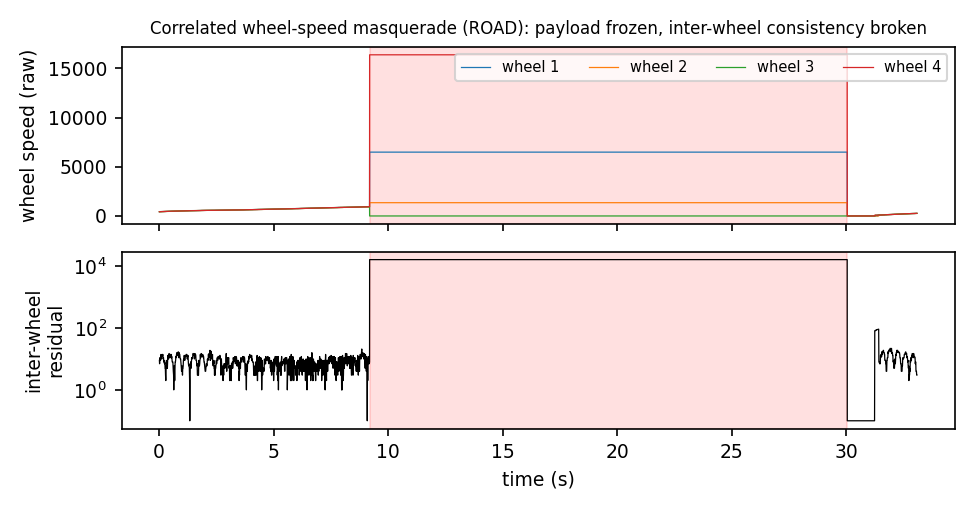
\includegraphics[width=\linewidth]{fig1_timeline.png}
\caption{Correlated wheel-speed masquerade (ROAD). Top: the four wheel-speed channels freeze at mutually inconsistent constants inside the injection interval (shaded). Bottom: the inter-wheel residual jumps from $\sim$10 to 16383.}
\label{fig:timeline}
\end{figure}

Table~\ref{tab:taxonomy} and Figure~\ref{fig:taxonomy} summarize all 26 injection captures. Every masquerade and fabrication class violates at least one law, and each class is identifiable by \emph{which} law it breaks. Wheel-speed masquerades break inter-wheel consistency (178--585$\times$) and continuity (258--1024$\times$). Speedometer masquerades break the display--wheel relation ($\sim$165$\times$) and mildly exceed the value envelope. Coolant masquerades exceed the envelope (255 vs.\ 151). The six reverse-light masquerades break nothing we can measure in these channels --- Section~5.3 explains why.

\begin{table}[t]
\centering
\small
\begin{tabular}{lcccc}
\toprule
Class (n) & L1 & L2 & L3 & L5/L6/L7 \\
\midrule
wheel masq.\ (3) & \textbf{178--585$\times$} & 84--659$\times$ & \textbf{258--1024$\times$} & --- \\
speedo masq.\ (3) & --- & \textbf{165$\times$} & --- & 1.3$\times$/6--11$\times$ \\
reverse-light masq.\ (6) & --- & --- & --- & \textbf{10--43$\times$ (L7)} \\
coolant masq.\ (1) & --- & --- & --- & \textbf{1.7$\times$ (L6)} \\
wheel fab.\ (3) & \textbf{178--585$\times$} & 86--984$\times$ & \textbf{258--1273$\times$} & --- \\
speedo fab.\ (3) & --- & --- & --- & \textbf{190--211$\times$ (L2d)} \\
reverse-light fab.\ (6) & --- & --- & --- & --- (evades) \\
\bottomrule
\end{tabular}
\caption{Physics taxonomy: maximum inside/outside residual ratio per class and law. Every class violates at least one law except reverse-light, which evades all measured channels. Fabrication numbers from our raw-log decoding (Section~7).}
\label{tab:taxonomy}
\end{table}

\begin{figure}[t]
\centering
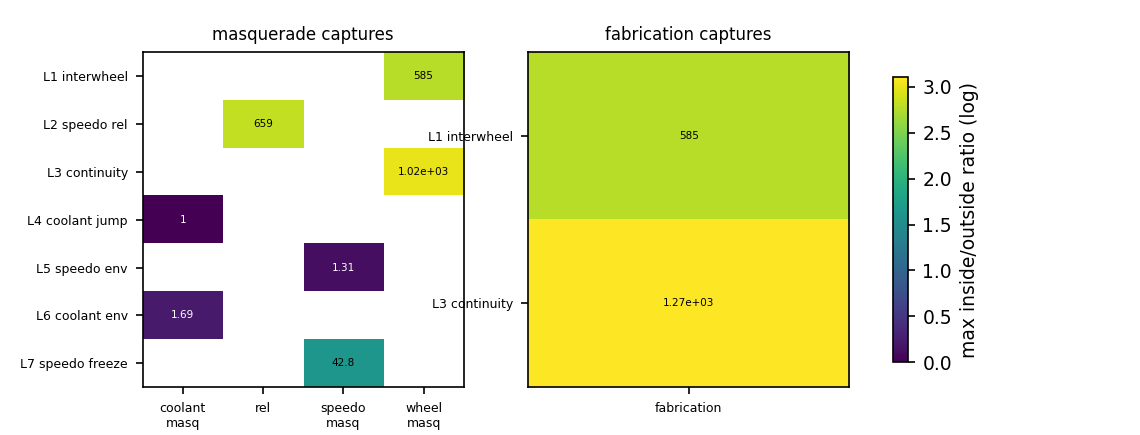
\includegraphics[width=\linewidth]{fig4_taxonomy.png}
\caption{Taxonomy heatmaps for both injection modes. Color: log$_{10}$ of the maximum inside/outside residual ratio per law and class.}
\label{fig:taxonomy}
\end{figure}

This taxonomy is itself useful: it tells a defender which sensor pairs to monitor for which threat model, and it bounds what physics can promise.

\textbf{Fabrication variants.} ROAD distributes each injection in two modes: a masquerade capture (fabricated frames replace suspended ones) and a fabrication capture (fabricated frames join the live traffic). We decoded all thirteen fabrication captures from the raw logs --- necessary because ROAD's shipped DBC does not reproduce its own published extractions (Section~7) --- and ran the same taxonomy. The results mirror the masquerades exactly: correlated fabrications break inter-wheel consistency (178--585$\times$) and continuity (258--1273$\times$); speedometer fabrications exceed the value envelope (16384 vs.\ a benign 573--1590) and jump the display relation (190--211$\times$); the six reverse-light fabrications evade every law, like their twins. Two consequences. First, ROAD's ``correlated'' fabrication --- advertised as the most stealthy fabrication possible in public data --- is not stealthy to physics: its injected wheel values are grossly inter-inconsistent once decoded with the correct layout (we reject our own pre-registered prediction here). Second, the reverse-light boundary is a property of the attack technique, not of one injection mode.

\section{Detector Ladder}
\subsection{Setup}
Frame-level scores on the attacked-ID stream. All thresholds come from the 99.9th percentile of ambient scores --- no attack data touches calibration. We report average precision and recall at that operating point, per class, with PR curves in Figure~\ref{fig:pr}.

\subsection{Results}
Table~\ref{tab:ladder} gives the comparison. Range statistics and kinematic residuals both catch the three payload classes perfectly (AP 0.97--1.0, recall 1.0); the payload values exceed ambient envelopes, so a plain range check suffices there. The constancy heuristic is dead on this dataset --- ambient stationary stretches produce runs of 106{,}279 identical frames, so it never fires. The interesting row is the reverse-light class: range statistics fail (AP 0.49), the constancy heuristic fails (0.34), and kinematic residuals fail (0.44).

\begin{table}[t]
\centering
\small
\begin{tabular}{lccc}
\toprule
Class & D0a range & D0b const-run & D1 physics \\
\midrule
wheel masq. & 0.999 / 1.00 & 0.995 / 0 & 0.999 / 1.00 \\
speedo masq. & 0.9995 / 1.00 & 0.42 / 0 & 0.995 / 1.00 \\
coolant masq. & 1.00 / 1.00 & 0.10 / 0 & 0.966 / 1.00 \\
reverse-light masq. & 0.49 / 0 & 0.34 / 0 & 0.44 / 0 \\
\midrule
\multicolumn{4}{l}{\emph{Stage 2 (capture-disjoint supervised):}} \\
wheel masq. & \multicolumn{2}{c}{RF 0.999 / XGB 0.999 / AE 0.997} & --- \\
speedo masq. & \multicolumn{2}{c}{RF 1.00 / XGB 1.00 / AE 0.99} & --- \\
coolant masq. & \multicolumn{2}{c}{RF 1.00 / XGB 0.165 / AE 0.747} & --- \\
reverse-light & \multicolumn{2}{c}{RF 0.37 / XGB 0.63 / \textbf{AE 0.975}} & --- \\
\bottomrule
\end{tabular}
\caption{Average precision / recall at the ambient-99.9th-percentile operating point. Stage 2 supervised models train on captures 1--2 of each class and test on capture 3; the AE trains on ambient frames only.}
\label{tab:ladder}
\end{table}

\begin{figure}[t]
\centering
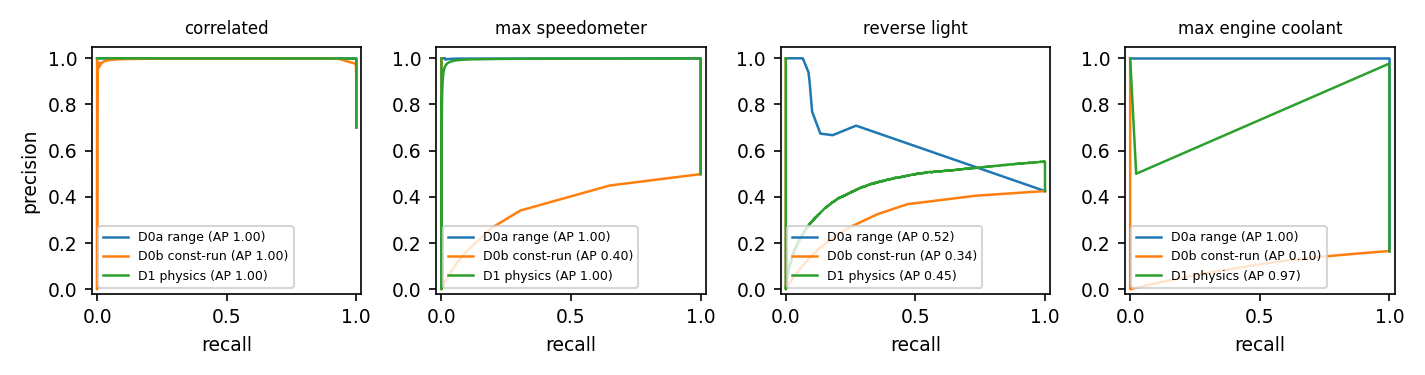
\includegraphics[width=\linewidth]{fig2_pr_stage1.png}
\caption{Precision--recall curves, stage 1, per class and detector.}
\label{fig:pr}
\end{figure}

\subsection{Why the Reverse-Light Masquerade Evades Physics}
The injector live-patches the light bit: the frame's rolling counter keeps incrementing during the attack (we measured maximum in-attack counter runs of one frame), and the patched frame is a snapshot taken at injection time. During those windows the vehicle moves steadily, so the frozen display value is consistent with the wheels. The attack is a \emph{dynamically consistent snapshot} --- physically valid at injection and for as long as the vehicle state does not change. Kinematics cannot flag it. A semantic law could (the light bit must agree with the gear), but ROAD's anonymized DBC hides the gear signal; our best guess fails on 48.6\% of ambient frames, so we report the class as open rather than force a broken detector.

Two supervised models confirm the difficulty: Random Forest generalizes across captures but reaches AP 0.37 on this class, XGBoost 0.63. The one-class autoencoder --- trained on ambient frames, never shown an attack --- ranks the class at AP 0.98, though at the strict ambient operating point its recall is near zero. The class is rankable, not thresholdable.

\section{Attribution: Does the Physics Constraint Pay?}
The remaining question is whether \emph{learning with physics} beats learning without it. We train a one-step wheel-speed forecaster twice: a PINN whose loss adds display-tracking and acceleration-limit terms, and an identical twin with the data loss only. Figure~\ref{fig:attr} shows average precision across four ambient training fractions.

\begin{figure}[t]
\centering
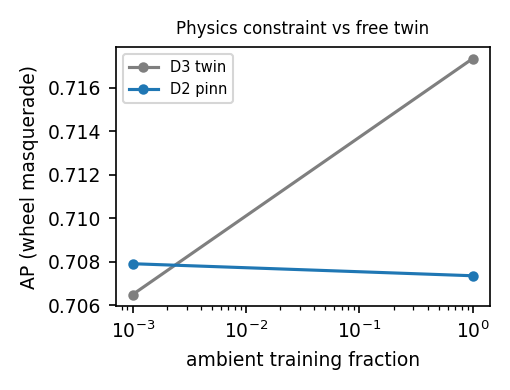
\includegraphics[width=0.85\linewidth]{fig3_attribution.png}
\caption{Attribution: PINN vs.\ physics-free twin across ambient training fractions. Parity everywhere; the twin edges ahead at 0.1\%.}
\label{fig:attr}
\end{figure}

The result is parity. At 100\% of the data, both reach AP 0.72. At 0.1\% (about a thousand frames), the twin edges ahead (0.726 vs.\ 0.714). A sweep of the physics weight $\lambda \in \{0.1, 1, 10\}$ moves nothing outside noise. Both models handle the accelerator captures --- real, unusual driving --- with zero false positives.

The mechanism is straightforward. The physics we can encode in a loss (display tracks wheels, speed changes smoothly) is a linear relation the twin learns from a thousand examples, and ROAD provides a million. This reproduces, in automotive security, the finding that physics priors pay off when the physics is hard to learn or the data is scarce~\cite{krishnapriyan2021,grossmann2024}. On this dataset, neither condition holds for the forecaster formulation. The physical knowledge that \emph{does} pay is the analytical form: it needs no training, no attack data, and it diagnoses \emph{which} law broke --- something a learned residual cannot name.

\section{Limitations}
ROAD's masquerade captures are simulated by post-processing, the vehicle ran on a dynamometer, and the frame ordering is deliberately obfuscated --- our timing features are weakened by the dataset's own design, and our claims are case-study evidence, not deployment results. A dataset-integrity finding deserves its own warning: the shipped anonymized DBC does not decode the published CSV signal extractions, and the bit layouts differ between capture families (four 14-bit fields in ambient extractions; 13/11/10/14 in masquerade extractions). We recovered the layouts empirically from log--CSV pairs and validated them by exact reproduction; anyone reusing ROAD's DBC will silently misdecode signals. One fabrication capture (coolant, $n{=}1$) has an unresolved decoding anomaly and is excluded from our claims. The gear signal required for a semantic reverse-light law is unrecoverable from the anonymized DBC. Our PINN encodes physics as soft constraints on a one-step forecaster; structural encodings (hard kinematic constraints, multi-step prediction) remain untested, so our negative attribution result is scoped to this formulation. Finally, the reverse-light finding may not transfer to a vehicle whose DBC exposes gear state --- the class is open on ROAD, not closed in general.

\section{Conclusion}
We asked where physics pays in the detection of CAN masquerade attacks, and measured the answer on the public benchmark. Kinematic residuals carry real information --- three of four masquerade classes at recall 1.0 with zero attack data, at ratios up to 1024$\times$ the benign envelope --- and they diagnose which law broke, which no learned detector offers. Learned soft-physics constraints add nothing here. One class evades everything value-based, physics-based, and supervised; a one-class autoencoder ranks it without seeing attacks. The wheels do tell the truth, most of the time --- and knowing exactly when they fall silent is what this paper adds.

\begin{thebibliography}{20}\small
\bibitem{verma2024} Verma, Bridges, Iannacone, et al., ``A comprehensive guide to CAN IDS data and introduction of the ROAD dataset,'' \emph{PLOS ONE} 19(1), 2024.
\bibitem{moriano2022} Moriano, Bridges, Iannacone, ``Detecting CAN masquerade attacks with signal clustering similarity,'' \emph{NDSS AutoSec}, 2022.
\bibitem{marfo2025} Marfo, Moriano, Tosh, Moore, ``Detecting masquerade attacks in controller area networks using graph machine learning,'' \emph{IEEE TIFS} 20, 2025.
\bibitem{moriano2026} Moriano, Hespeler, Li, Bridges, ``Evaluating lightweight unsupervised online IDS for masquerade attacks in CAN,'' \emph{JISA} 98, 2026.
\bibitem{song2026} Song, Ahn, Baek, Kim, Kim, Jeon, ``AutoHack: a physically verified multi-bus CAN dataset for IDS evaluation,'' \emph{USENIX VehicleSec}, 2026.
\bibitem{hoppe2007} Hoppe, Dittmann, ``Vort\"auschen fahrzeuginterner CAN-Kommunikation,'' VDI/VW Automotive Security, 2007.
\bibitem{koscher2010} Koscher, Czeskis, Roesner, et al., ``Experimental security analysis of a modern automobile,'' \emph{IEEE S\&P}, 2010.
\bibitem{miller2013} Miller, Valasek, ``Adventures in automotive networks and control units,'' DEF CON 21, 2013.
\bibitem{serag2025} Serag et al., ``SoK: kicking CAN down the road,'' arXiv:2510.02960, 2025.
\bibitem{rahman2026} Rahman, Salek, Chowdhury, ``Digital twin-based intrusion detection for vehicle powertrain CAN bus systems,'' arXiv:2608.17093, 2026.
\bibitem{wasicek2017} Wasicek, Pes\'e, Weimerskirch, et al., ``Context-aware intrusion detection in automotive control systems,'' escar, 2017.
\bibitem{muter2010} M\"uter, Groll, Freiling, ``A structured approach to anomaly detection for in-vehicle networks,'' IAS, 2010.
\bibitem{axelsson2000} Axelsson, ``The base-rate fallacy and its implications for the difficulty of intrusion detection,'' \emph{ACM TISSEC} 3(3), 2000.
\bibitem{arp2022} Arp et al., ``Dos and don'ts of machine learning in computer security,'' \emph{USENIX Security}, 2022.
\bibitem{tatbul2018} Tatbul et al., ``Precision and recall for time series,'' \emph{NeurIPS}, 2018.
\bibitem{kim2022} Kim et al., ``Towards a rigorous evaluation of time-series anomaly detection,'' \emph{AAAI}, 2022.
\bibitem{road2020} ``Real ORNL Automotive Dynamometer (ROAD) CAN intrusion dataset,'' Zenodo 10462796, 2020.
\bibitem{krishnapriyan2021} Krishnapriyan et al., ``Characterizing possible failure modes in physics-informed neural networks,'' \emph{NeurIPS}, 2021.
\bibitem{grossmann2024} Grossmann et al., ``Can physics-informed neural networks beat the finite element method?'' \emph{ICLR}, 2024.
\bibitem{jabbari2023} Jabbari Zideh et al., ``Physics-informed convolutional autoencoder for cyber anomaly detection in power distribution grids,'' arXiv:2312.04758, 2023.
\end{thebibliography}

\end{document}
